 \chapter[Referencial teórico]{Referencial teórico}\label{sec-revisao}

Neste capítulo, revisamos a literatura, os conceitos e as ferramentas que fundamentam este trabalho.
Primeiramente, passamos brevemente pela inferência causal tradicional (com covariáveis, indicadora de intervenção e desfecho escalares) no arcabouço de resultados potenciais \cite{rubin_estimating_1974, holland_statistics_1986}.
Introduzimos sua extensão para o contexto funcional-temporal, com ênfase no nosso estimando de interesse, o \(\mathrm{FATE}\) \cite{ecker_causal_2024}; e falamos sobre propostas correlatas \cite{testa_doubly-robust_2025, sparkes_functional_2024}.
Em seguida, discutimos ondaletas sob a ótica da análise multirresolução \cite{mallat_theory_1989, vidakovic_statistical_1999} e do \emph{lifting scheme} \cite{sweldens_lifting_1995}, além de aludirmos a trabalhos que discorram sobre o processamento de funções por ondaletas em tempo real \cite{liu_improved_2014}.

\section{Inferência causal}\label{sec-inferencia-causal}

Estimar um efeito causal é, no fundo, comparar um cenário que efetivamente ocorreu, com um que teria ocorrido sob um curso de ação diferente.
Esta seção apresenta o arcabouço que torna esse problema tratável e as suposições sob as quais um efeito causal pode ser recuperado a partir de dados puramente observados.
Tratamos aqui do caso em que o desfecho do indivíduo é um valor escalar. A extensão para trajetórias funcionais é retomada na Seção \ref{sec-inferencia-causal-funcional}.

Uma forma particularmente útil de organizar o problema causal é recorrer à estrutura de resultados potenciais, que explicita o caráter contrafactual do desfecho de interesse. 
Considere um estudo com \(i = 1, \dots, N\) participantes, em que cada indivíduo, a quem se atribui um tratamento \(A_i \in \mathcal{A} \equiv \{0, 1\}\), apresenta um vetor de \(P\) covariáveis pré-tratamento \(\mathbf{X}_i\) (com realização \(\mathbf{x}_i\)) e um desfecho mensurado \(Y_i\). 
No modelo tradicionalmente atribuído a Neyman e Rubin \cite{rubin_estimating_1974, holland_statistics_1986}, associamos a cada indivíduo dois resultados potenciais, \(Y_i^{(1)}\) e \(Y_i^{(0)}\). 
Esses resultados representam o que o i-ésimo indivíduo teria experienciado caso tivesse, respectivamente, recebido ou não o tratamento \((A_i = 1, A_i = 0)\). 
Como o efeito causal é definido a partir dessas quantidades contrafactuais, ele só é identificável (em sentido causal; não confundir com a identificabilidade estatística usual, em que valores distintos do parâmetro geram distribuições distintas) se puder ser reescrito como uma função da distribuição dos dados observados \((\mathbf{X}, A, Y)\). 
As suposições a seguir são o que viabilizam a passagem do contrafactual ao observável:

\begin{enumerate}
    \item Ausência de confundimento não mensurado (também chamada de ignorabilidade condicional):
	\[
            \{Y_i^{(a)}: a \in \mathcal{A}\} \perp A_i \mid \mathbf{X}_i.
    \]
    
    Implica que, uma vez condicionada às covariáveis \(\mathbf{X}_i\), a atribuição de tratamento \(A_i\) é ``como se'' aleatória e, portanto, não carrega informação adicional sobre os desfechos potenciais. 
    Para tanto, \(\mathbf{X}_i\) deve conter as confundidoras, isto é, as variáveis que afetam tanto a atribuição do tratamento \(A_i\) quanto o desfecho \(Y_i\).

    \item Positividade (ou sobreposição): denotando por \(\pi_a(\mathbf{X}_i) = \mathbb{P}(A_i = a \mid \mathbf{X}_i)\) a propensão do i-ésimo indivíduo ao tratamento \(a \in \mathcal{A}\), requeremos, conforme \citeonline{rosenbaum_central_1983}, 
		\[
            0 < \pi_a(\mathbf{X}_i) < 1, \quad \forall a \in \mathcal{A}, \ \text{q.c.}
        \]

    Em palavras, para valores de \(\mathbf{X}_i\) que ocorrem com probabilidade positiva, deve haver chance não nula de observar cada nível de tratamento. 
    Essa restrição garante que os grupos dos distintos níveis de intervenção sejam comparáveis.

    \item Consistência: para cada resultado potencial, digamos, \(Y_i^{(a)}\), se, de fato, \(A_i = a\), então \(Y_i^{(A_i)} = Y_i^{(a)} = Y_i\); para tratamento binário, isso equivale a \(Y_i = A_i Y_i^{(1)} + (1 - A_i) Y_i^{(0)}\). 
    Apesar de parecer intuitiva, essa suposição assegura a não existência de múltiplas versões dum mesmo tratamento \(a\) que conduzam a diferentes desfechos potenciais. 
    O que pode ser difícil de garantir em algumas aplicações \cite{hernan_causal_2023}.

    \item Ausência de interferência: postula que os desfechos potenciais do i-ésimo indivíduo dependem apenas do seu próprio tratamento. 
    Em especial, para \(i \neq j\), a atribuição \(A_j\) não afeta \(Y_i^{(a)}\) (assumindo, ademais, uma única versão de tratamento).\footnote{As suposições (3) e (4) são, em conjunto, chamadas de SUTVA (\emph{Stable Unit Treatment Value Assumption}, em português: Suposição de Valor de Tratamento de Unidade Estável).} Essa condição pode falhar, por exemplo, em estudos de vacinação, em que imunizar uma parcela considerável da população reduz o risco de infecção também entre os não vacinados (imunidade de rebanho).  
\end{enumerate}

Em experimentos aleatorizados, a aleatorização costuma tornar plausíveis as suposições de ignorabilidade condicional e de positividade; ainda assim, a consistência e a ausência de interferência dependem do desenho e da definição da intervenção. Em estudos observacionais, por sua vez, a consistência, a ausência de confundimento não mensurado e a ausência de interferência são tipicamente não testáveis a partir dos dados, ao passo que violações de positividade podem ser parcialmente diagnosticadas empiricamente (por exemplo, via distribuição do escore de propensão).

Garantidas essas quatro condições, podemos estimar, entre outros possíveis efeitos causais de interesse, o ATE (\emph{Average Treatment Effect}, em português: Efeito Médio de Tratamento):
\begin{equation}
    \mathrm{ATE} = \mathbb{E}[Y^{(1)} - Y^{(0)}] = \mathbb{E}[Y^{(1)}] - \mathbb{E}[Y^{(0)}],
    \label{eq:ate_def}
\end{equation}
através de métodos que, em grande medida, buscam recuperar sob diferentes suposições e desenhos, as quantidades \(\mathbb{E}[Y^{(1)}]\) e \(\mathbb{E}[Y^{(0)}]\).
Diferenças em diferenças, modelos de regressão, métodos baseados em pareamento, modelos marginais e, mais recentemente, métodos de aprendizado de máquina adaptados à inferência causal são algumas das abordagens propostas pela literatura para estimar o ATE e análogos, como o CATE (\emph{Conditional Average Treatment Effect}, em português: Efeito Médio Condicional de Tratamento) e o ATT (\emph{Average Treatment Effect on the Treated}, em português: Efeito Médio de Tratamento nos Tratados) \cite{rubin_estimating_1974, imbens_causal_2015, hernan_causal_2023, nogueira_methods_2022, yao_survey_2021, chernozhukov_doubledebiased_2018, athey_estimating_2019}. 

Em situações menos tradicionais (quando nos afastamos do cenário com uma única intervenção e variáveis escalares fixas, para considerar estruturas mais ricas de dados e intervenções), podemos ter covariáveis e desfecho, por exemplo, variando no tempo, além de múltiplas atribuições de tratamento. 
\citeonline{hernan_causal_2023} discutem extensivamente métodos de inferência causal para dados longitudinais, com ênfase em como a complexidade adicional do contexto longitudinal se reflete na necessidade de suposições mais fortes. 

No contexto funcional, a literatura ainda está em fase embrionária \cite{belloni_program_2017, ecker_causal_2024, wong_kernel-based_2018, colantuoni_statistical_2018, sparkes_functional_2024}. 
Apesar de o trabalho de \citeonline{ying_causality_2024} fornecer condições teóricas para uma análise causal longitudinal completamente funcional (covariáveis, indicadora de tratamento e desfecho), esse tipo de formulação ainda é, sobretudo, um referencial do que seria necessário para uma generalização plena do caso escalar. 
Na prática, é comum que os requisitos e objetos envolvidos sejam mais fortes do que usualmente conseguimos justificar ou aproximar empiricamente. 
Por essa razão, a literatura aplicada em inferência causal funcional, até então, tem privilegiado extensões parciais do caso escalar, nas quais apenas uma parte do tripé \((\mathbf{X}, A, Y)\) é funcional. 
\citeonline{ecker_causal_2024}, por exemplo, estenderam a estrutura de resultados potenciais assumindo apenas desfechos (incluindo os desfechos potenciais) funcionais.

\subsection{FATE e Inferência causal funcional}\label{sec-inferencia-causal-funcional}

No trabalho de \citeonline{ecker_causal_2024}, para cada indivíduo \(i = 1, \dots, N\) e período \(t \in \mathcal{T}\), denotamos por \(Y_i^{(1)}(t)\) e \(Y_i^{(0)}(t)\) as curvas dos desfechos potenciais sob tratamento e controle, respectivamente; \(\mathcal{T}\) corresponde ao período de acompanhamento após a intervenção.
Considerando o exemplo que trouxemos no Capítulo \ref{sec-introducao}, \(Y_i^{(1)}(t)\) representaria a curva de consumo do domicílio \(i\) caso este recebesse a tarifa dinâmica, e \(Y_i^{(0)}(t)\), a curva que este mesmo domicílio apresentaria caso recebesse a tarifa padrão.
\(A_i\) indicaria qual das duas tarifas foi efetivamente atribuída, enquanto \(\mathbf{X}_i\) representaria as características socioeconômicas do domicílio.

As suposições necessárias à identificabilidade do \(\mathrm{FATE}\) são análogas às do caso escalar. A ignorabilidade condicional, todavia, é relaxada pelos autores em favor da ignorabilidade média.\footnote{Enquanto a ignorabilidade condicional (Seção \ref{sec-inferencia-causal}) exige \({Y^{(a)}} \perp A \mid \mathbf{X}\) em nível distribucional, a ignorabilidade média requer apenas a igualdade das esperanças condicionais. 
A condição plena identifica qualquer funcional da distribuição dos desfechos potenciais (média, variância, quantis), ao passo que a ignorabilidade média identifica apenas a média de \(Y\). 
Como o \(\mathrm{FATE}\) é uma média, a versão mais fraca é suficiente.} 
Em suma, em vez de assumirmos uma independência em termos distribucionais, requeremos que, para todo \(t\),
\[
    \mathbb{E}[Y^{(a)}(t) \mid A, \mathbf{X}] = \mathbb{E}[Y^{(a)}(t) \mid \mathbf{X}],
    \quad a \in \mathcal{A} \equiv \{0, 1\}.
\]

Sob essas condições, a identificabilidade do parâmetro causal funcional, \(\mathrm{FATE} \equiv \theta(t)\), segue a lógica pontual:
\begin{equation}
\begin{aligned}
    \theta(t)
    &= \mathbb{E}\big[Y^{(1)}(t)\big] - \mathbb{E}\big[Y^{(0)}(t)\big] \\
    &\overset{\text{(i)}}{=} \mathbb{E}\Big[\mathbb{E}\big[Y^{(1)}(t) \mid \mathbf{X}\big] - \mathbb{E}\big[Y^{(0)}(t) \mid \mathbf{X}\big]\Big] \\
    &\overset{\text{(ii)}}{=} \mathbb{E}\Big[\mathbb{E}\big[Y^{(1)}(t) \mid A = 1, \mathbf{X}\big] - \mathbb{E}\big[Y^{(0)}(t) \mid A = 0, \mathbf{X}\big]\Big] \\
    &\overset{\text{(iii)}}{=} \mathbb{E}\Big[\mathbb{E}\big[Y(t) \mid A = 1, \mathbf{X}\big] - \mathbb{E}\big[Y(t) \mid A = 0, \mathbf{X}\big]\Big].
    \label{eq:fate_identificabilidade}
\end{aligned}
\end{equation}

As igualdades decorrem, respectivamente, das esperanças iteradas e da linearidade da esperança (i), da ignorabilidade média (ii) e da consistência (iii); a positividade garante que as esperanças condicionais em \(A = a\) estejam bem definidas.

Ao assumir que apenas os desfechos variam no tempo, \citeonline{ecker_causal_2024} introduzem um modelo de regressão linear funcional \cite{ramsay_functional_2005} para estimar cada uma das esperanças condicionais em \ref{eq:fate_identificabilidade}. 
Os autores ajustam separadamente dois modelos; um utilizando apenas os indivíduos tratados (\(A = 1\)) e outro utilizando apenas os do grupo controle (\(A = 0\)). 
A abordagem assume que os parâmetros variam suavemente ao longo do tempo, viabilizando, consequentemente, sua representação via bases de expansão globais. 

Seja \(N_a\) o número de indivíduos no nível de tratamento \(a \in \{0, 1\}\), \(\boldsymbol{\beta}^{(a)}(t)\) o vetor de parâmetros funcionais que mensura a influência das covariáveis \(\mathbf{X}\) (para a população que recebeu a intervenção \(a\)), e \(\epsilon_i^{(a)}(t)\) um termo de erro estocástico. 
Supondo que \(\mathbf{X}_i \in \mathbb{R}^{P}\) inclui o intercepto, para cada nível de intervenção \(a \in \{0, 1\}\), temos:
\begin{equation}
    Y_i^{(a)}(t) = \mathbf{X}_i^{\mathsf{T}}\boldsymbol{\beta}^{(a)}(t) + \epsilon_i^{(a)}(t), \quad \text{para } i \text{ tal que } A_i = a.
    \label{eq:ecker_modelo_regressao_funcional}
\end{equation}

Em \ref{eq:ecker_modelo_regressao_funcional}, vale dizer que o superescrito \((a)\) indica que cada desfecho potencial carrega seu próprio erro, cuja distribuição pode diferir entre os grupos; não implica que a intervenção seja a causa do erro. 
Assumimos que o vetor de erros \(\boldsymbol{\epsilon}^{(a)}(t)\) segue um MGP (\emph{Multivariate Gaussian Process}, em português: Processo Gaussiano Multivariado), denotado por \(\mathrm{MGP}(\mathbf{0}, \sigma_a, \mathcal{I}_{N_a})\), em que \(\mathcal{I}_{N_a}\) é a matriz identidade de dimensão \(N_a \times N_a\). 
Essa especificação implica independência entre indivíduos, mas modela explicitamente a correlação temporal para um mesmo sujeito através da função de covariância \(\sigma_a(s,t) = \mathrm{Cov}\left(\epsilon_i^{(a)}(s), \epsilon_i^{(a)}(t)\right)\), para \(s, t \in \mathcal{T}\), garantindo que \(\mathbb{E}[Y_i^{(a)}(t) \mid \mathbf{X}_i] = \mathbf{X}_i^{\mathsf{T}}\boldsymbol{\beta}^{(a)}(t)\), o que conecta o modelo às esperanças condicionais em \eqref{eq:fate_identificabilidade}.

O efeito \(\theta(t)\) é, então, estimado em dois passos. Primeiro, calculamos, para cada indivíduo, as duas predições contrafactuais geradas pelos modelos ajustados nos grupos tratado e controle (usando \(\hat{\boldsymbol{\beta}}^{(1)}(t)\) e \(\hat{\boldsymbol{\beta}}^{(0)}(t)\)). 
Em seguida, tomamos a diferença média dessas predições em toda a amostra, conforme a Equação \ref{eq:ecker_estimador_fate},
\begin{equation}
    \hat{\theta}(t) = \frac{1}{N}\sum\limits_{i = 1}^{N}\left(\mathbf{X}_i^{\mathsf{T}}\hat{\boldsymbol{\beta}}^{(1)}(t) - \mathbf{X}_i^{\mathsf{T}}\hat{\boldsymbol{\beta}}^{(0)}(t)\right) = \bar{\mathbf{X}}^{\mathsf{T}}\left(\hat{\boldsymbol{\beta}}^{(1)}(t) - \hat{\boldsymbol{\beta}}^{(0)}(t)\right).
    \label{eq:ecker_estimador_fate}
\end{equation}

Julgamos importante reforçar que o modelo definido na Equação \ref{eq:ecker_modelo_regressao_funcional} (e, consequentemente, o estimador em \ref{eq:ecker_estimador_fate}) pressupõe o acesso às trajetórias contínuas \(Y_i(t)\). 
Na prática, entretanto, é comum observarmos apenas dados discretos e ruidosos. Essa discrepância, como já adiantado no Capítulo \ref{sec-introducao}, impõe uma etapa de representação funcional geralmente anterior ao ajuste do modelo (embora menos comum, também é possível aplicar a suavização aos resultados do modelo ajustado \cite{testa_doubly-robust_2025}). 
Operacionalmente, \citeonline{ecker_causal_2024} primeiro suavizam as curvas observadas e depois ajustam os modelos via mínimos quadrados ordinários (ponto a ponto) sobre os objetos funcionais resultantes.

Em nossa proposta, essa suavização será realizada por ondaletas, sendo cada curva \(Y_i[k]\) suavizada individualmente pela DWT com limiarização antes de alimentar o modelo de regressão funcional. 
No exemplo da rede elétrica, isso equivale a suavizar a série de consumo de cada domicílio separadamente.

Cabe ressaltar que os autores também propuseram bandas simultâneas de confiança de nível \((1 - \alpha)\%\) para \(\hat{\theta}(t)\), dadas por
\begin{equation}
    \hat{\theta}(t) \pm u_{\alpha}(t)\sqrt{C_{\theta}(t, t)},
    \label{eq:ecker_bandas_simultaneas}
\end{equation}
em que \(C_{\theta}(s, t) = \sigma_{1}(s, t)\bar{\mathbf{X}}^{\mathsf{T}}\left(\mathbf{X}_{1}^{\mathsf{T}}\mathbf{X}_{1}\right)^{-1}\bar{\mathbf{X}} + \sigma_{0}(s, t)\bar{\mathbf{X}}^{\mathsf{T}}\left(\mathbf{X}_{0}^{\mathsf{T}}\mathbf{X}_{0}\right)^{-1}\bar{\mathbf{X}}\), e \(u_{\alpha} = \{u_{\alpha}(t): t \in \mathcal{T}\}\) é uma função de limiarização tal que, para um dado nível \(\alpha\),
\[
    \mathbb{P}\left(\theta(t) \in \hat{\theta}(t) \pm u_{\alpha}(t)\sqrt{C_{\theta}(t, t)}, \quad \forall t \in \mathcal{T}\right) \geq 1 - \alpha. 
\]

O que dá validade às coberturas simultâneas da Equação \ref{eq:ecker_bandas_simultaneas} é a premissa de que o estimador \(\hat{\theta}(t)\) preserva a natureza gaussiana do processo gerador de dados. 
Dado que o ajuste via mínimos quadrados ordinários constitui uma operação linear nas observações, \(\hat{\theta}(t)\) converge para um processo gaussiano (pois assumimos que \(\boldsymbol{\epsilon}^{(a)}(t)\) segue um \(\mathrm{MGP}\)). 
É com base nessa propriedade linear que resultados clássicos da teoria de campos aleatórios podem ser utilizados para calibrar o limiar \(u_{\alpha}(t)\). 
Tal garantia teórica, no entanto, perde-se quando o procedimento de estimação incorpora etapas não lineares --- como a limiarização de coeficientes em ondaletas ou a seleção adaptativa de hiperparâmetros de suavização --- exigindo justificativas adicionais em abordagens que priorizam esparsidade ou adaptação a descontinuidades locais.
Tendo isso em vista, cabe ressaltar que, em seu trabalho, \citeonline{ecker_causal_2024} fixaram o número de bases das \textit{B-splines} e não recorreram à validação cruzada generalizada. 

Em uma vertente paralela que busca relaxar a dependência estrita de processos gaussianos, \citeonline{sparkes_functional_2024} também reivindicam a formalização do \(\mathrm{FATE}\). 
Eles, porém, trabalham com uma filosofia de estimação distinta, focada na robustez distributiva. 
Em sua proposta, os autores introduzem a ``classe \(\mathcal{U}\)''. 

Tome \(Z\) como uma variável aleatória limitada, com suporte \(S_Z \subset \mathbb{R}\). 
Definimos a média funcional de \(Z\) por \(\mathrm{Av}(Z) \equiv |S_Z|^{-1} \int_{S_Z} z \, dz\), em que \(|S_Z|\) denota a medida de Lebesgue do suporte. 
Dizemos que \(Z\) pertence à classe \(\mathcal{U}\) se, e somente se, sua esperança coincide com sua média funcional. 
Isto é, \(\mathbb{E}[Z] = \mathrm{Av}(Z)\). 
A partir dessa definição, \citeonline{sparkes_functional_2024} propõem substituir as suposições clássicas pela premissa de que o desfecho potencial condicional, \(Y^{(a)}(t) \mid \mathbf{X}\), pertence à classe \(\mathcal{U}\) para todo \(a \in \{0,1\}\). 
Sob tais condições, os autores argumentam que a identificação do efeito causal funcional torna-se mais tolerante a desvios das premissas tradicionais.

Em essência, a proposta de \citeonline{sparkes_functional_2024} desloca o papel de suposições de independência probabilística (como a ignorabilidade condicional) para hipóteses adicionais sobre a geometria e a distribuição dos dados. 
A condição de pertinência à classe \(\mathcal{U}\) é satisfeita, por exemplo, por distribuições simétricas (como uma Normal truncada simetricamente ou uma Uniforme), mas pode ser inadequada em aplicações nas quais os desfechos apresentam assimetria ou caudas mais pesadas, situação recorrente em contextos biológicos e econômicos. 
Somado a isso, a hipótese de que \(Y^{(a)}(t)\) pertence à classe \(\mathcal{U}\) não é diretamente verificável para o desfecho contrafactual não observado. 
Assim, embora a proposta forneça uma alternativa potencialmente útil em cenários com amostragem informativa ou confundimento residual, sua aplicação depende de uma regularidade distributiva tão difícil de se atestar quanto a das hipóteses causais clássicas de Neyman--Rubin.


Em uma outra direção que também busca maior robustez, agora, focada na proteção contra a má especificação de modelos, \citeonline{testa_doubly-robust_2025} discutem uma alternativa fundamentada na teoria semiparamétrica. 
Em linhas gerais, a proposta estende a lógica de estimadores duplamente robustos, consolidada na inferência causal escalar \cite{imbens_causal_2015}, para o domínio funcional. 
O método combina um modelo para a atribuição de tratamento via escore de propensão, \(\pi(\mathbf{X}) = \mathbb{P}(A = 1\mid \mathbf{X})\), e um modelo de regressão para o desfecho funcional, \(\mu_a(\mathbf{X}, t) = \mathbb{E}[Y^{(a)}(t)\mid \mathbf{X}]\); e os utiliza conjuntamente para formar um pseudo desfecho que tem como objetivo a redução de viés.

Uma consequência prática dessa construção é que a estimativa obtida ponto a ponto ao longo de \(t \in \mathcal{T}\) tende a apresentar grande variabilidade, sobretudo quando os pesos associados ao escore de propensão se tornam instáveis (sintoma frequente de sobreposição limitada). 
Para contornar esse problema e recuperar a regularidade funcional, \citeonline{testa_doubly-robust_2025} aplicam a suavização diretamente sobre a trajetória desse pseudo desfecho robusto, contrastando com a prática usual de suavizar previamente os dados observados. 
Ainda que seja uma escolha natural do ponto de vista da construção do estimador, em aplicações práticas com dados brutos discretos, esparsos ou contaminados por ruído de medição, não empregar o pré-processamento antes de modelar pode ser uma estratégia perigosa. 
A recuperação prévia da trajetória latente \(Y_i(t)\) (pré-processamento) costuma ser importante para garantir a estabilidade numérica do ajuste de modelos funcionais, pois ruídos de medição não tratados podem se propagar para as fases de modelagem e inferência.

Completamos nosso panorama da inferência causal funcional ao mencionar propostas que abordam estimandos distintos do \(\mathrm{FATE}\), ou lidam com estruturas de dados alternativas. 
\citeonline{wong_kernel-based_2018}, por exemplo, focam na estimação de um efeito escalar (\(\mathrm{ATE}\)) ajustado por covariáveis funcionais, utilizando balanceamento via \emph{kernel}. 
\citeonline{colantuoni_statistical_2018} tratam de desfechos funcionais sujeitos a censura informativa (como curvas de sobrevida ou qualidade de vida interrompidas por óbito). 
Já \citeonline{kikuchi_dynamic_2025} expande a definição de intervenção, investigando efeitos de trajetórias de exposição no espaço-tempo. 
Por fim, propostas como as de \citeonline{belloni_high-dimensional_2014} estabelecem o arcabouço teórico para a inferência em alta dimensão.

Como já pontuado (Capítulo \ref{sec-introducao}), a estimação de efeitos causais funcionais se beneficiaria de um pré-processamento capaz de lidar com descontinuidades locais e ruído sem recorrer a informação de instantes futuros. 
Introduzimos, a seguir, o arcabouço teórico das transformadas por ondaletas; técnica de suavização/filtragem que utilizaremos para este fim.

\section{Ondaletas}

Ondaletas são funções que satisfazem certas propriedades. Elas oscilam ao longo do que, para nós, será o tempo \(t \in \mathcal{T}\) e pertencem ao espaço de funções quadrado integráveis \(\mathrm{L}^{2}(\mathbb{R})\) (isto é, possuem ``energia'' finita) \cite{morettin_wavelets_2017, vidakovic_statistical_1999}.

Uma dada função \(\psi(t)\) é uma ondaleta se satisfizer:
\begin{enumerate}
  \item Condição de média nula: \(\int_{-\infty}^{\infty} \psi(t) dt = 0\). Garante que a função seja oscilatória, com áreas positivas e negativas que se cancelam.\footnote{A condição de média nula implica que \(\hat{\psi}(0) = 0\) (em que \(\hat{\psi}\) é a transformada de Fourier de \(\psi\)). Em construções usuais, essa propriedade é suficiente para a admissibilidade (isto é, para que \(\int_0^\infty \left(|\hat{\psi}(\omega)|^2/|\omega|\right) d\omega < \infty\)), condição que garante que a CWT (\emph{Continuous Wavelet Transform}, em português: Transformada de Ondaletas Contínua) seja estavelmente inversível.} É a propriedade que torna as ondaletas sensíveis a flutuações e mudanças na função que queremos representar, digamos, \(f(t)\).

  \item Energia finita: \(\int_{-\infty}^{\infty} |\psi(t)|^{2} dt < \infty\). Formaliza a noção de que a ondaleta é uma perturbação localizada, no sentido de que sua energia se concentra em torno de uma região do domínio (tipicamente com decaimento à medida que \(|t|\) cresce). 

\end{enumerate}

A Figura \ref{fig:onda_comparacao_seno_mexican_hat} exibe a ondaleta de Haar, definida por \(\psi_{\text{Haar}}(t) = \mathbb{I}_{[0, 1/2)}(t) - \mathbb{I}_{[1/2, 1)}(t)\), com \(\mathbb{I}\) denotando a função indicadora, e a ondaleta chapéu mexicano, \(\psi_{\text{Chapéu Mex.}}(t) = (1 - t^2) \exp\{-t^2/2\}\). Para fins de visualização, ambas estão representadas na figura transladadas para \(t=10\) e dilatadas. É fácil ver que uma função como \(\sin(t)\) respeita somente a condição (1), enquanto as ondaletas, como as da Figura \ref{fig:onda_comparacao_seno_mexican_hat}, satisfazem, simultaneamente, as condições (1) e (2).

\begin{figure}[!ht]
	\centering
	\begin{subfigure}{0.48\textwidth}
    	\centering
    	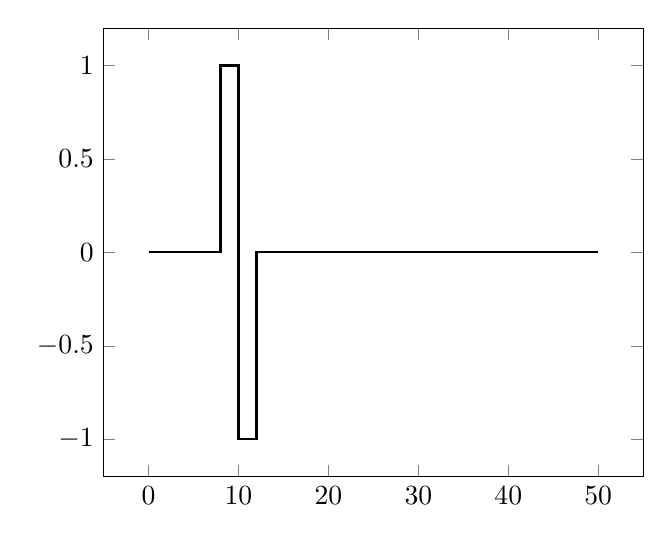
\begin{tikzpicture}
        	\begin{axis}
        		\addplot[
		            % color=royalblue, 
        		    domain=0:50,
            		samples=500,
            		thick,
		        ] coordinates {
		            (0,0) (8,0)       % Zero até t=8
		            (8,1) (10,1)      % Sobe para 1 de 8 a 10
        		    (10,-1) (12,-1)   % Desce para -1 de 10 a 12
            		(12,0) (50,0)     % Zero de 12 em diante
        		};
        	\end{axis}  
    	\end{tikzpicture}
    	\caption{Ondaleta de Haar.}
	    \label{fig:onda_haar}
	\end{subfigure}
	\hfill
	\begin{subfigure}{0.48\textwidth}
    	\centering
    	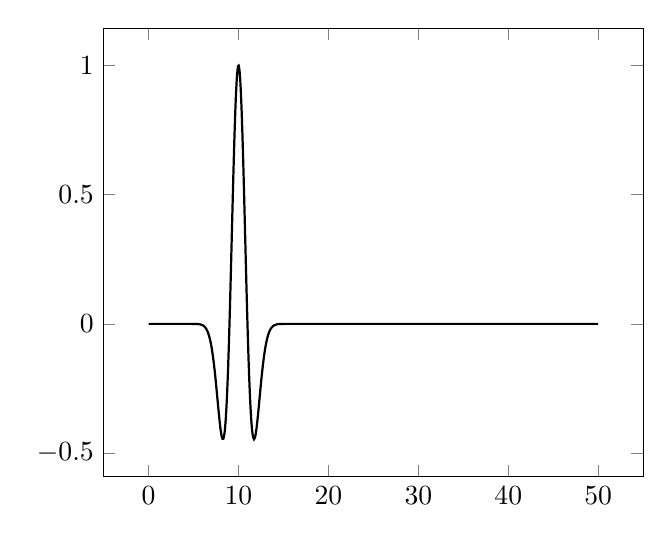
\begin{tikzpicture}
	        \begin{axis}
	        % Gráfico da Wavelet "Mexican Hat"
	        \addplot[
	            % color=royalblue,
	            domain=0:50,
	            samples=500,
	            smooth,
	            thick,
	        ] {(1 - (x-10)^2) * exp(-(x-10)^2 / 2)};
	        \end{axis} 
	    \end{tikzpicture}
    	\caption{Ondaleta chapéu mexicano.}
	    \label{fig:onda_mexican_hat}
	\end{subfigure}
	\caption{Ondaletas de Haar e chapéu mexicano.}
	\label{fig:onda_comparacao_seno_mexican_hat}
\end{figure}

As ondaletas apresentam vantagens frente a métodos globais de decomposição de funções, como os \emph{B-splines}, sobretudo na representação de descontinuidades e picos.
Para precisar essa vantagem, caracterizamos antes a noção de regularidade que empregaremos ao longo do texto.

\begin{definition}[Regularidade de Hölder]\label{def:regularidade}
    Seja \(t_0\) um ponto do domínio de \(f\) e seja \(\alpha \geq 0\). Dizemos que \(f\) é \(\alpha\)-regular em \(t_0\) se existirem uma constante \(C > 0\) e um polinômio \(P\) de grau \(\lfloor \alpha \rfloor\) tais que
    \[
        |f(t) - P(t - t_0)| \leq C\,|t - t_0|^{\alpha}
    \]
    em uma vizinhança de \(t_0\).
    Se a desigualdade vale com o mesmo \(C\) para todo \(t_0\), dizemos que \(f\) é uniformemente \(\alpha\)-regular \cite{mallat_wavelet_2009}.
\end{definition}

O expoente \(\alpha\) quantifica a suavidade local de \(f\) em torno de \(t_0\) e pode variar de ponto a ponto, sendo alto onde a função se aproxima de um polinômio e baixo onde há picos ou descontinuidades (um salto corresponde a \(\alpha = 0\)).
Uma representação por \emph{B-splines} ajusta seus coeficientes a partir de toda a extensão do sinal, o que exige que o efeito subjacente seja uniformemente regular.
Reforça-se que, como pontuado no Capítulo \ref{sec-introducao}, supor tal regularidade é especialmente delicado em inferência causal, pois o efeito de tratamento não é observado e sua regularidade não pode ser conferida a partir dos dados, ainda que os desfechos observados pareçam regulares.
Havendo trechos não uniformemente regulares, uma resolução global única não os acomoda sem suavizar em excesso as demais regiões.
A limiarização em ondaletas, por operar coeficiente a coeficiente, ajusta-se à regularidade local e concentra esses comportamentos em poucos coeficientes de detalhe, desempenho que estimadores lineares, como os \emph{B-splines}, não alcançam \cite{donoho_ideal_1994}.

No exemplo da rede elétrica, a curva de consumo de cada domicílio tende a concentrar sua irregularidade em horários específicos de alta demanda, permanecendo estável nos demais períodos. É exatamente esse tipo de estrutura que as ondaletas capturam com naturalidade, adaptando a resolução local ao nível de irregularidade de cada trecho.

Para melhor entender como as ondaletas são utilizadas na decomposição de funções, é conveniente introduzir a série e a transformada de Fourier.

\subsection{Série de Fourier} \label{sec:fourier_series}
Suponha que temos o interesse em uma função de período \(L\) definida em \(\mathrm{L}^{2}([c, c + 2L])\), \(f(t)\), que satisfaz certas condições de regularidade (conhecidas como condições de Dirichlet). A série de Fourier postula que é possível expandir \(f(t)\) através de um coeficiente de base, e uma combinação linear infinita de senos e cossenos com frequências cada vez maiores \cite{guidorizzi_um_2013}. Formalmente, 
\begin{equation}
  f(t) = \frac{a_0}{2} + \sum\limits_{n = 1}^{\infty} \left[a_n \cos\left(\frac{nt\pi}{L}\right) + b_n \sin\left(\frac{nt\pi}{L}\right)\right],
  \label{eq:fourier_serie_real}
\end{equation}
em que \(a_0, a_n\) e \(b_n \in \mathbb{R}\), \(\forall n\), variam de acordo com a função \(f(t)\) que será representada.

Note que o fato de \(f(t)\) ser expansível por uma combinação linear se relaciona com a ideia de decomposição em bases que aparece em espaços vetoriais de dimensão finita \(\left(\mathbb{R}^{n}, n < \infty\right)\). Aqui, porém, essa noção é transportada para o espaço de funções, e as bases em que a função é decomposta passam a ser funções trigonométricas. Outra característica interessante da Equação \ref{eq:fourier_serie_real} reside nos termos \(a_n\) e \(b_n\). Esses termos quantificam o quanto \(f(t)\) se aproxima das funções-base \(\cos\left(nt\pi/L\right)\) e \(\sin\left(nt\pi/L\right)\), e são obtidos pela generalização do produto escalar para o espaço de funções, o produto interno.

Na Equação \ref{eq:fourier_coeficientes}, apresentamos as expressões para a obtenção de \(a_0, a_n\) e \(b_n\). Vale notar que o termo \(a_0/2\) na expansão da série de Fourier equivale ao valor médio da função \(f(t)\) no intervalo considerado \((c, c + 2L)\). Uma vez que o nível médio (ou o deslocamento vertical) da função é capturado por \(a_0/2\), todo o somatório de senos e cossenos se encarrega de modelar exclusivamente as oscilações e flutuações de \(f(t)\) em torno dessa média. Em suma, a série de Fourier primeiro estabelece o ``nível de base'' da função e, em seguida, adiciona todas as componentes oscilatórias necessárias para reconstruir sua forma detalhada:
\begin{equation}
  \begin{aligned}
      a_0 &= \frac{1}{L}\int_{c}^{c + 2L} f(t) dt \\
      a_n &= \frac{1}{L}\int_{c}^{c + 2L} f(t)\cos\left(\frac{n\pi t}{L}\right) dt \\
      b_n &= \frac{1}{L}\int_{c}^{c + 2L} f(t)\sin\left(\frac{n\pi t}{L}\right) dt.
  \end{aligned}
  \label{eq:fourier_coeficientes}
\end{equation}

Uma forma alternativa e equivalente para a série de Fourier pode ser obtida utilizando a fórmula de Euler. Na Equação \ref{eq:fourier_serie_complexa} apresentamos esta expressão, que é mais próxima da notação utilizada na transformada de Fourier, e nas análises de ondaletas: 
\begin{equation}
  f(t) = \sum_{n=-\infty}^{\infty} c_n e^{i \frac{n\pi t}{L}}
  \label{eq:fourier_serie_complexa}
\end{equation}
Nesta representação, o somatório agora se estende por todos os inteiros, e os coeficientes \(c_n\) são números complexos que contêm a informação tanto de amplitude quanto de fase de cada componente de frequência (é fácil mostrar que eles estão diretamente relacionados com \(a_n\) e \(b_n\)). 

A forma complexa (Equação \ref{eq:fourier_serie_complexa}) é sempre equivalente à forma real (Equação \ref{eq:fourier_serie_real}) para funções \(f(t)\) de valor real. 

\subsection{Transformada de Fourier}\label{sec:fourier_transform} 
Até agora, restringimos \(f(t)\) para que tivesse período \(L\). Se utilizássemos a série de Fourier para decompor, por exemplo, o chapéu mexicano da Figura \ref{fig:onda_mexican_hat}, o processo assumiria que a função se repete a cada \(2L\) (o tamanho do intervalo), forçando uma representação periódica da ondaleta. A Figura \ref{fig:fourier_series_mexican_hat} apresenta essa noção visualmente. 

\begin{figure}[!ht]
	\centering
	\begin{subfigure}{0.48\textwidth}
		\centering
	    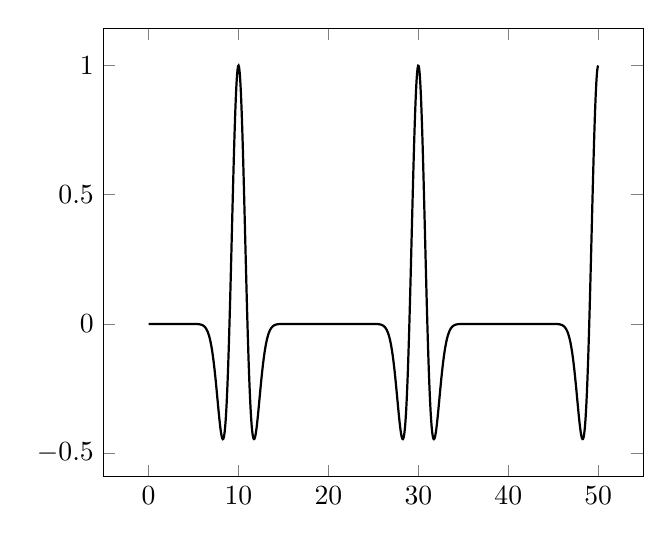
\begin{tikzpicture}
	        \begin{axis}
	        \addplot[
	            domain=0:50,
	            samples=1000,
	            smooth,
	            thick,
	        ] {(1 - (mod(x, 20)-10)^2) * exp(-(mod(x, 20)-10)^2 / 2)};
	        \end{axis}
	    \end{tikzpicture}
	    \caption{Representação do chapéu mexicano pela série de Fourier.}
	    \label{fig:fourier_series_mexican_hat}
	\end{subfigure}
	\hfill 
	\begin{subfigure}{0.48\textwidth}
	    \centering
	    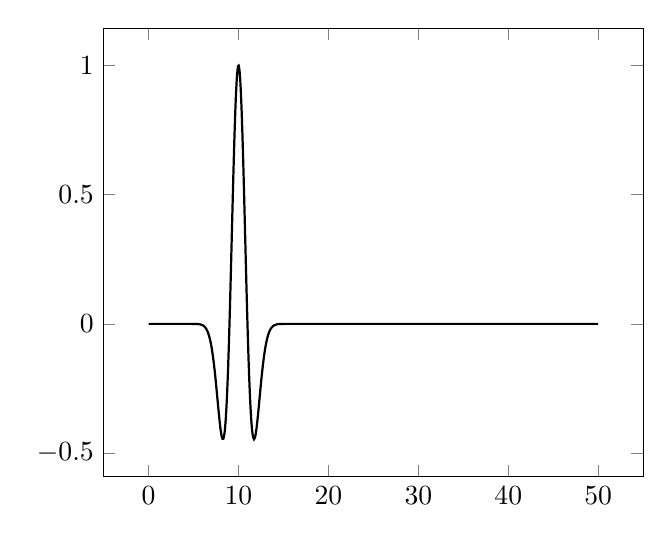
\begin{tikzpicture}
	        \begin{axis}
	        \addplot[
	            domain=0:50,
	            samples=500,
	            smooth,
	            thick,
	        ] {(1 - (x-10)^2) * exp(-(x-10)^2 / 2)};
	        \end{axis}
	    \end{tikzpicture}
	    \caption{Ondaleta chapéu mexicano original (não periódica).}
	    \label{fig:mexican_hat}
	\end{subfigure}
	\caption{A série de Fourier força uma representação periódica (esquerda) para uma função que é inerentemente localizada e não periódica (direita).}
	\label{fig:fig_2_fourier_mexican_hat}
\end{figure}

Para superar essa limitação, a transformada de Fourier trata uma função não periódica como se o período desta fosse infinito. Considere a forma complexa da série de Fourier (Equação \ref{eq:fourier_serie_complexa}). Seja \(\omega_n = n\pi/L\) a frequência angular do n-ésimo harmônico. O espaçamento entre duas frequências consecutivas é, então, \(\Delta\omega = \omega_{n+1} - \omega_n = \pi/L\). Podemos reescrever o coeficiente \(c_n\) da série complexa em termos de \(\Delta\omega\). Como \(L = \pi/\Delta\omega\), temos
\begin{equation*}
    c_n = \frac{1}{2L}\int_{-L}^{L} f(t) e^{-i \omega_n t} dt = \frac{\Delta\omega}{2\pi}\int_{-L}^{L} f(t) e^{-i \omega_n t} dt.
\end{equation*}
Agora, substituímos essa expressão na soma da série de Fourier:
\begin{equation*}
    f(t) = \sum_{n=-\infty}^{\infty} c_n e^{i \omega_n t} = \frac{1}{2\pi} \sum_{n=-\infty}^{\infty} \left[
      \int_{-L}^{L} f(\zeta) e^{-i \omega_n \zeta} d\zeta \right] e^{i \omega_n t} \Delta\omega.
\end{equation*}

Quando fazemos o período da série tender a infinito (\(L \to \infty\)), o espaçamento entre as frequências se torna infinitesimal (\(\Delta\omega \to 0\)) e o intervalo de integração \([-L, L]\) se expande para \(\mathbb{R}\). Heuristicamente, \(f(t)\) pode ser expressa pelo limite de uma soma de Riemann,
\begin{equation*}
    f(t) = \lim_{\Delta\omega \to 0} \frac{1}{2\pi} \sum_{n=-\infty}^{\infty} \left[
      \int_{-L}^{L} f(\zeta) e^{-i \omega_n \zeta} d\zeta \right] e^{i \omega_n t} \Delta\omega.
\end{equation*}
Neste limite, o somatório se transforma em uma integral, \(\Delta\omega\) se torna o diferencial \(d\omega\) e a frequência discreta \(\omega_n\) se torna a variável contínua \(\omega\). 

A expressão dentro dos colchetes se torna uma função contínua de \(\omega\), que definimos como a transformada de Fourier de \(f(t)\) \cite{vidakovic_statistical_1999}:
\begin{equation}
    F(\omega) = \int_{-\infty}^{\infty} f(\zeta) e^{-i\omega \zeta} d\zeta.
    \label{eq:eq_5_fourier_transform}
\end{equation}
A soma inteira converge para a integral que reconstrói a função original, conhecida como a transformada inversa de Fourier:
\begin{equation*}
    f(t) = \frac{1}{2\pi} \int_{-\infty}^{\infty} F(\omega) e^{i\omega t} d\omega.
\end{equation*}

A transformada e a transformada inversa de Fourier podem ser utilizadas conjuntamente para transitar entre o domínio do tempo, \(f(t)\), e o domínio da frequência, \(F(\omega)\). Não podemos utilizá-las, no entanto, para localizar em quais momentos do tempo cada componente de frequência ocorre (veja sobre o princípio da incerteza de Heisenberg-Gabor \cite{heisenbergBerAnschaulichenInhalt1927}). Abordagens como a STFT (\emph{Short-Time Fourier Transform}, em português: Transformada de Fourier de Tempo Curto) lidam com este problema, grosso modo, aplicando uma transformada de Fourier a janelas temporais de tamanho fixo. Se as janelas temporais são muito estreitas, temos uma boa resolução temporal, mas uma má resolução de frequência (a análise de frequência é imprecisa, pois a janela captura poucas oscilações). Todavia, se a janela temporal é larga, temos uma boa resolução de frequência (a transformada tem um segmento longo para analisar, resultando em picos de frequência nítidos), mas uma má resolução temporal.

A resolução tempo-frequência uniforme da STFT é inadequada para sinais complexos que contêm simultaneamente eventos de alta frequência e curta duração (que demandariam uma janela temporal estreita) e eventos de baixa frequência e longa duração (que demandariam uma janela larga). As ondaletas lidam com este problema empregando uma janela temporal que se adapta à natureza da função, com alta resolução temporal para analisar eventos rápidos e alta resolução de frequência para analisar eventos lentos. 

A Figura \ref{fig:fig_3_stft_wavelet_tiling} ilustra a diferença das janelas temporais adotadas pela STFT e pelas decomposições baseadas em ondaletas.

\begin{figure}[!ht]
	\centering
	\begin{subfigure}{0.48\textwidth}
	    \centering
	    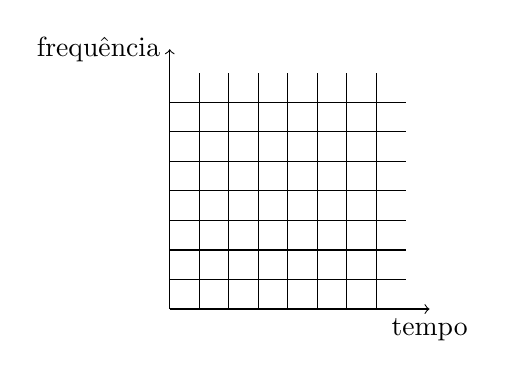
\begin{tikzpicture}[scale=1.5]
	        \draw[->] (0,0) -- (2.2,0) node[below] {tempo};
	        \draw[->] (0,0) -- (0,2.2) node[left] {frequência};
	      
	        \foreach \x in {0.25, 0.5, 0.75, 1, 1.25, 1.5, 1.75}
	            \draw (\x, 0) -- (\x, 2);
	        \foreach \y in {0.25, 0.5, 0.75, 1, 1.25, 1.5, 1.75}
	            \draw (0, \y) -- (2, \y);
	    \end{tikzpicture}
	    \caption{Grade tempo-frequência da STFT.}
	    \label{fig:fig_3_stft}
	\end{subfigure}
	\hfill 
	\begin{subfigure}{0.48\textwidth}
	    \centering
	    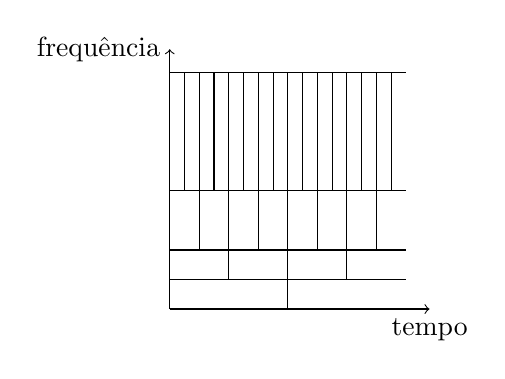
\begin{tikzpicture}[scale=1.5]
	        \draw[->] (0,0) -- (2.2,0) node[below] {tempo};
	        \draw[->] (0,0) -- (0,2.2) node[left] {frequência};
	        \draw (0, 0.25) -- (2, 0.25);
	        \draw (1, 0) -- (1, 0.25);
	        \draw (0, 0.5) -- (2, 0.5);
	        \draw (0.5, 0.25) -- (0.5, 0.5);
	        \draw (1, 0.25) -- (1, 0.5);
	        \draw (1.5, 0.25) -- (1.5, 0.5);
	        \draw (0, 1) -- (2, 1);
	        \foreach \x in {0.25, 0.5,..., 1.75}
	            \draw (\x, 0.5) -- (\x, 1);
	        \foreach \x in {0.125, 0.25,..., 1.875}
	            \draw (\x, 1) -- (\x, 2);
	        \draw (0, 2) -- (2, 2);
	    \end{tikzpicture}
	    \caption{Grade tempo-frequência das ondaletas.}
	    \label{fig:fig_3_wavelet}
	\end{subfigure}
	\caption{Comparação da resolução tempo-frequência. A STFT (esquerda) possui resolução fixa, enquanto as ondaletas (direita) possuem resolução adaptativa.}
	\label{fig:fig_3_stft_wavelet_tiling}
\end{figure}

\subsection{Transformada por ondaletas}
Tal como a série e a transformada de Fourier, a análise por ondaletas representa uma função \(f(t) \in \mathrm{L}^{2}(\mathbb{R})\) como uma combinação linear de funções mais simples. A diferença consiste no fato de que essas funções não são senoides de frequências distintas, mas translações e dilatações de uma única função geradora, a ondaleta-mãe, \(\psi(t)\). 

A família de funções geradas por \(\psi(t)\) é composta por transformações de translação (ou deslocamento) e escala (ou dilatação). A operação de translação, controlada por um parâmetro \(b\) \((\psi(t-b))\), desloca a ondaleta ao longo do eixo do tempo, permitindo que a análise se concentre em diferentes momentos da função. Essa flexibilidade favorece a localização temporal. Por outro lado, a transformação de escala, controlada por um parâmetro \(a > 0\) \((\psi(t/a))\), dilata ou comprime a ondaleta. Na análise de ondaletas, as noções de escala e frequência estão inversamente relacionadas: escalas grandes (\(a > 1\)) correspondem a uma ondaleta dilatada, que oscila mais lentamente, e são utilizadas para capturar características de baixa frequência; escalas pequenas (\(a < 1\)), por sua vez, correspondem a uma ondaleta comprimida, que oscila rapidamente, e são utilizadas para detectar picos, descontinuidades e mudanças abruptas. Combinando essas duas operações, a família de ``ondaletas-filhas'', \(\psi_{a,b}(t)\), é gerada de acordo com:
\begin{equation}
    \psi_{a,b}(t) = \frac{1}{\sqrt{a}} \psi\left(\frac{t-b}{a}\right).
    \label{eq:eq_6_wavelet_family}
\end{equation}
O fator de normalização \(1/\sqrt{a}\) garante que a energia de cada ondaleta-filha permaneça constante, independentemente da escala, o que permite que os coeficientes de diferentes escalas sejam diretamente comparáveis.

Denotando por \(\overline{\psi}\) o conjugado complexo de \(\psi\), podemos decompor \(f(t)\) por ondaletas através da CWT, definida pelos coeficientes \(W(a, b)\) dados pela Equação \ref{eq:eq_7_cwt} \cite{vidakovic_statistical_1999}:
\begin{equation}
    W(a,b) = \int\limits_{-\infty}^{\infty} f(t) \frac{1}{\sqrt{a}} \overline{\psi}\left(\frac{t-b}{a}\right) dt.
    \label{eq:eq_7_cwt}
\end{equation}

Embora teoricamente elegante, na prática, a CWT não costuma ser a técnica empregada em análises por ondaletas. 
Devido ao seu caráter contínuo, os coeficientes \(W(a, b)\) costumam ser redundantes e são caros de serem obtidos computacionalmente. 
Nesse sentido, as transformadas por ondaletas são geralmente implementadas de modo discreto, via MRA (\emph{Multiresolution Analysis}, em português: Análise Multirresolução), e chamadas de DWT (\emph{Discrete Wavelet Transform}, em português: Transformada de Ondaletas Discreta).

\subsubsection{Transformada de ondaletas discreta e análise multirresolução}\label{sec-dwt-mra}

A DWT, realização discreta e computacional da análise por ondaletas, tem como arcabouço matemático a MRA.
Nesta, decompomos o espaço de funções de energia finita em uma sequência de subespaços fechados aninhados, denotados por \(\{V_{2^j}\}_{j \in \mathbb{Z}}\), com \(j\) representando o nível de resolução do subespaço (quanto maior \(j\), mais fina a resolução). 
Formalmente, dizemos que cada subespaço \(V_{2^j}\) contém a aproximação da função original \(f(t)\) na resolução \(2^j\). 
Conforme definido por \citeonline{mallat_theory_1989}, requeremos que a sequência de subespaços satisfaça:
\begin{enumerate}
    \item \(V_{2^j} \subset V_{2^{j+1}}, \forall j \in \mathbb{Z}\).
    Significa que a aproximação de uma função \(f(t)\) em uma resolução \(2^{j + 1}\) contém toda a informação necessária para calcular a mesma função em uma resolução menor (como \(2^{j}\)).

    \item \[
    	\lim_{j \rightarrow \infty} V_{2^j} = \bigcup_{j \in \mathbb{Z}} V_{2^j} \text{ é densa em } \mathrm{L}^2(\mathbb{R}),
    \]
    \[
    	\lim_{j \rightarrow -\infty} V_{2^j} = \bigcap_{j \in \mathbb{Z}} V_{2^j} = \{0\}.
    \]
    Implica que, conforme \(j \to +\infty\), a aproximação no subespaço \(V_{2^{j}}\) converge para a função original; e, por outro lado, quando \(j \to -\infty\), a aproximação perde toda a informação e converge para zero.

    \item \(f(t) \in V_{2^j} \iff f(2t) \in V_{2^{j + 1}}, \forall j \in \mathbb{Z}\).
    Implica que as operações de aproximação são similares em todas as resoluções, de modo que os subespaços das funções aproximadas podem ser derivados uns dos outros a partir de operações de dilatação.

    \item \(f(t) \in V_{2^j} \implies f(t - 2^{-j} n) \in V_{2^j}, \forall n, j \in \mathbb{Z}\).
    Garante que cada subespaço seja invariante por translações proporcionais à sua escala (\(2^{-j}\)); em particular, no nível de referência (\(j = 0\)) recupera-se a invariância por translações inteiras, propriedade necessária para que a aproximação de \(f(t)\) possa ser obtida a partir de amostras discretas igualmente espaçadas.

    \item existe uma função de escala \(\phi \in V_{2^0}\) tal que \(\{\phi(t - n)\}_{n \in \mathbb{Z}}\) é base ortonormal de \(V_{2^0}\).
\end{enumerate}

Ao combinar as condições 3 e 5, a família
\begin{equation}
    \left\{ \phi_{j,n}(t) = \sqrt{2^{j}} \, \phi(2^j t - n) \right\}_{n \in \mathbb{Z}}
    \label{eq:base_funcao_escala}
\end{equation}
forma uma base ortonormal de \(V_{2^{j}}\) \(\forall j \in \mathbb{Z}\), e não apenas no nível de referência.
Como resultado, a aproximação de \(f(t)\) na resolução \(2^j\), denotada por \(f_{2^{j}}(t)\), pode ser escrita através da projeção ortogonal de \(f(t)\) sobre essa base,
\begin{equation}
    f_{2^j}(t) = \sum_{n = -\infty}^{+\infty} \underbrace{\left( \int_{-\infty}^{+\infty} f(\tau) \phi_{j,n}(\tau) \, d\tau \right)}_{s_j[n]} \phi_{j,n}(t).
    \label{eq:mra_approximation}
\end{equation}

Por construção, a aproximação \(f_{2^{j}}(t)\) não captura a informação contida em subespaços de maior resolução.
Isto é, como \(V_{2^j} \subset V_{2^{j+1}}\) e \(f_{2^{j}}(t) \in V_{2^j}\), a informação que diferencia \(V_{2^j}\) de \(V_{2^{j + 1}}\) não lhe é acessível.
Esse conteúdo, a que chamamos de detalhes, reside no complemento ortogonal, \(O_{2^j}\), de \(V_{2^j}\) em \(V_{2^{j+1}}\): \(V_{2^{j+1}} = V_{2^j} \;\oplus\; O_{2^j}\).

Assim como a função de escala \(\phi\) gera os subespaços de aproximação (Equação \ref{eq:base_funcao_escala}), cada subespaço de detalhe \(O_{2^j}\) é gerado por uma ondaleta-mãe, \(\psi\), que, por sua vez, depende diretamente de \(\phi\), conforme a Equação \ref{eq:filtros} \citeonline{mallat_theory_1989},
\begin{equation}
    \begin{aligned}
        \phi(t) &= \sqrt{2} \sum_{m \in \mathbb{Z}} h[m] \, \phi(2t - m), \\
        \psi(t) &= \sqrt{2} \sum_{m \in \mathbb{Z}} g[m] \, \phi(2t - m).
    \end{aligned}
    \label{eq:filtros}
\end{equation}
Aqui, os coeficientes \(h[m]\) e \(g[m]\) são chamados, respectivamente, de filtros passa-baixa e passa-alta. Conquanto os tenhamos escrito no nível de referência (\(j = 0\)), por conta da condição 3, os dois filtros relacionam \(V_{2^j}\) a \(V_{2^{j+1}}\) para todo \(j \in \mathbb{Z}\).

Com isso, a família
\begin{equation}
    \left\{ \psi_{j,n}(t) = \sqrt{2^{j}} \, \psi(2^j t - n) \right\}_{n \in \mathbb{Z}}
    \label{eq:wavelets_basis}
\end{equation}
constitui uma base ortonormal de \(O_{2^j}\) (desde que a transformada de Fourier de \(\psi\) guarde uma relação determinada com a de \(\phi\). Veja \citeonline{bachman_fourier_2000} para mais detalhes).
Agora, de modo análogo ao que fizemos para as aproximações (Equação \ref{eq:mra_approximation}), os detalhes de \(f(t)\) na resolução \(2^j\) são dados por
\begin{equation}
    d_{2^j}(t) = \sum_{n = -\infty}^{+\infty} \underbrace{\left( \int_{-\infty}^{+\infty} f(\tau) \psi_{j,n}(\tau) \, d\tau \right)}_{d_j[n]} \psi_{j,n}(t),
    \label{eq:mra_details}
\end{equation}
de tal sorte que \(s_j[n]\) e \(d_j[n]\) (Equações \ref{eq:mra_approximation} e \ref{eq:mra_details}) determinam inteiramente \(f_{2^j}(t)\) e \(d_{2^j}(t)\) e, consequentemente, a representação de \(f(t)\) no \((j + 1)\)-ésimo nível de resolução.

Neste ponto, surge a questão de como obter os coeficientes \(s_j[n]\) e \(d_j[n]\) na prática. As integrais em \ref{eq:mra_approximation} e \ref{eq:mra_details} exigem o conhecimento da função \(f(t)\) em toda a extensão do domínio, o que raramente é possível.
Geralmente, em vez dessa curva contínua, observamos apenas um sinal discreto \(f[k]\) (\(k \in \{0, 1, \dots, T-1\}\), \(T \in \mathbb{N}\)), em geral ruidoso, amostrado em pontos de \(\mathcal{T}\); a relação entre esse sinal e a função latente é formalizada na Seção \ref{sec-limiarizacao}.

Para aplicarmos a DWT e obtermos os coeficientes nesse cenário, é necessário assumir que o sinal discreto \(f[k]\) já constitui os coeficientes de aproximação no nível mais fino disponível, digamos, \(J\). Isto é, \(s_J[\kappa] = f[k]\) (passamos a indexar as sequências discretas por \(\kappa\), reservando \(n\) para as translações contínuas das bases).
Sob essa premissa, e graças à invariância por escala, os coeficientes dos níveis mais grosseiros (\(j < J\)) decorrem recursivamente dos mais finos, sem o cálculo de qualquer integral.
Mais concretamente, partindo da aproximação em uma resolução mais fina \(s_{j+1}[\kappa]\), conseguimos obter os coeficientes do nível imediatamente mais grosseiro pela Equação \ref{eq:algoritmo_piramidal} \cite{mallat_theory_1989},
\begin{equation}
    \begin{aligned}
        s_{j}[\kappa] &= \sum_{m \in \mathbb{Z}} h[m-2\kappa] \, s_{j+1}[m], \\
        d_{j}[\kappa] &= \sum_{m \in \mathbb{Z}} g[m-2\kappa] \, s_{j+1}[m].
    \end{aligned}
    \label{eq:algoritmo_piramidal}
\end{equation}

A seguir, ilustramos a mecânica da DWT via MRA, para uma única resolução (\(J - 1\)), com um exemplo simples, utilizando a ondaleta de Haar. 
\begin{example}[DWT via MRA com a ondaleta de Haar]
    Considere o sinal discreto \(f[k] = [3, 4, 5, 6, 1, 2, 3, 4]\). 
    De acordo com o que foi pontuado anteriormente, assumiremos que este sinal representa os coeficientes de aproximação na escala mais fina, isto é, \(s_{J}[\kappa] = f[k]\) (no nível mais fino, \(\kappa\) coincide com o índice \(k\)), com \(j \leq J \in \mathbb{Z}\). 
    Aplicaremos um nível de decomposição para obter \(s_{J-1}\) e \(d_{J-1}\).

    Para a ondaleta de Haar, utilizamos os filtros \(h = [1/\sqrt{2}, 1/\sqrt{2}]\) e \(g = [1/\sqrt{2}, -1/\sqrt{2}]\). 
    Como os filtros de Haar têm apenas dois coeficientes não nulos, o somatório da Equação \ref{eq:algoritmo_piramidal} reduz-se, para cada \(\kappa\), a \(s_{J-1}[\kappa] = h[0]\,s_J[2\kappa] + h[1]\,s_J[2\kappa + 1]\) (e analogamente para \(d_{J-1}\), com o filtro \(g\)). 
    O deslocamento \(2\kappa\) corresponde à subamostragem, responsável por cada coeficiente consumir um par distinto de amostras consecutivas, como se vê a seguir.
    \begin{itemize}
        \item A aproximação (\(s_{J-1}\)) é obtida a partir de \(s_J[\kappa]\) e do filtro \(h\):
        \begin{align*}
            s_{J-1}[0] &= h[0]s_J[0] + h[1]s_J[1] \approx 0.7071(3) + 0.7071(4) \approx 4.95 \\
            s_{J-1}[1] &= h[0]s_J[2] + h[1]s_J[3] \approx 0.7071(5) + 0.7071(6) \approx 7.78 \\
            s_{J-1}[2] &= h[0]s_J[4] + h[1]s_J[5] \approx 0.7071(1) + 0.7071(2) \approx 2.12 \\
            s_{J-1}[3] &= h[0]s_J[6] + h[1]s_J[7] \approx 0.7071(3) + 0.7071(4) \approx 4.95 \\
            s_{J-1} &\approx [4.95, 7.78, 2.12, 4.95].
        \end{align*}

        \item Os detalhes (\(d_{J-1}\)) são calculados analogamente, mas com base no filtro \(g\):
        \begin{align*}
            d_{J-1}[0] &= g[0]s_J[0] + g[1]s_J[1] \approx 0.7071(3) - 0.7071(4) \approx -0.71 \\
            d_{J-1}[1] &= g[0]s_J[2] + g[1]s_J[3] \approx 0.7071(5) - 0.7071(6) \approx -0.71 \\
            d_{J-1}[2] &= \dots \approx -0.71 \\
            d_{J-1}[3] &= \dots \approx -0.71 \\
            d_{J-1} &\approx [-0.71, -0.71, -0.71, -0.71].
        \end{align*}
        
    \end{itemize}
\end{example} 

Poderíamos utilizar \(s_{J - 1}\) para continuar a iteração do algoritmo para níveis de resolução mais grosseiros. 
Poderíamos, ainda, empregar outras ondaletas para decompor o mesmo sinal. 
A ondaleta Daubechies 2 (também conhecida como \texttt{db2} ou \texttt{d4}), por exemplo, possui filtros passa-baixa e passa-alta com coeficientes aproximadamente iguais a
\[
	h \approx [0.483, 0.836, 0.224, -0.129] \text{ e } g \approx [-0.1294, -0.2241, 0.8365, -0.4830].
\]
O uso de ondaletas associadas a filtros mais longos, contudo, tende a agravar problemas na representação das bordas do sinal. 
Discutiremos algumas das possíveis soluções para isso na Seção \ref{sec-extensoes-borda}.

\subsection{Lifting scheme}\label{sec-lifting-scheme}
O processo descrito na Seção \ref{sec-dwt-mra} refere-se à implementação clássica e amplamente difundida da DWT. 
Trata-se da abordagem predominante na literatura estatística, sendo comumente encontrada em pacotes do ambiente R, como o \texttt{wavethresh}, o \texttt{wavelets} e o \texttt{waveslim} \cite{nason_wavethresh_1999, aldrich_wavelets_2005, brandon_whitcher_waveslim_2001}. 
Existem, entretanto, abordagens alternativas. 
Proposto por \citeonline{sweldens_lifting_1995} e posteriormente consolidado por \citeonline{daubechies_factoring_1998}, o \emph{lifting scheme} representa uma forma mais moderna e flexível de aplicar a DWT.

Em termos gerais, no \emph{lifting scheme}, para a resolução máxima \(J\) (com \(j \leq J, j \in \mathbb{Z}\)), aplicamos quatro operadores ao sinal \(f[k]\), assumindo — tal como na Seção \ref{sec-dwt-mra} — que o vetor de aproximação inicial \(s_{J}[\kappa]\) é idêntico a \(f[k]\). 
Assumiremos ainda que o sinal tem um número par de observações \(T\); caso o número seja ímpar, aplicamos tratamentos de borda, como na Seção \ref{sec-extensoes-borda}. 
Os operadores são: separação (\emph{split}), predição (\emph{prediction}), atualização (\emph{update}) e normalização (\emph{scaling}). 
O operador de separação divide \(s_{J}[\kappa]\) em dois subconjuntos disjuntos, \(s_{J, \text{par}}[\kappa] = s_{J}[2\kappa]\), contendo os elementos de índices pares, e \(s_{J, \text{ímpar}}[\kappa] = s_{J}[2\kappa + 1]\), contendo os de índices ímpares. 
Por exemplo, para o sinal \(f[k] = [3,4,5,6,1,2,3,4]\), e assumindo a indexação padrão iniciada em 0, temos \(s_{J, \text{par}}[\kappa] = [3, 5, 1, 3]\) (índices \(0, 2, 4, 6\)) e \(s_{J, \text{ímpar}}[\kappa] = [4, 6, 2, 4]\) (índices \(1, 3, 5, 7\)). 
Por construção, espera-se que as componentes pares e ímpares sejam altamente correlacionadas, justificando o uso de \(s_{J, \text{par}}\) para tentar predizer \(s_{J, \text{ímpar}}\). 
Utilizamos, assim, um operador de predição \(\mathcal{P}\) (que dependerá, entre outras coisas, da ondaleta escolhida para a decomposição da função) e chamamos os erros dessa predição de ``detalhe'' (análogos aos detalhes da Equação \ref{eq:algoritmo_piramidal}):
\begin{equation}
\begin{aligned}
    \hat s_{J,\text{ímpar}}[\kappa] &= \mathcal{P}\!\big(s_{J, \text{par}}[\kappa]\big),\\
    d_{J-1}[\kappa] &= s_{J, \text{ímpar}}[\kappa] - \hat s_{J, \text{ímpar}}[\kappa].
\end{aligned}
\label{eq:lifting-predictor-detail}
\end{equation}

É possível que a subamostra \(s_{J, \text{par}}[\kappa]\), sofra de falseamento (\emph{aliasing}) e falhe em preservar propriedades globais do sinal, tais como a sua média. 
Para corrigir isso, introduzimos um operador de atualização \(\mathcal{U}\), que ajusta a aproximação com base nos detalhes recém-calculados na Equação \ref{eq:lifting-predictor-detail}:
\begin{equation}
    s_{J-1}[\kappa] = s_{J, \text{par}}[\kappa] + \mathcal{U}\!\big(d_{J-1}[\kappa]\big).
\end{equation}

Após a atualização, é comum aplicar uma etapa de normalização, reescalando \(s_{J-1}[\kappa]\) e \(d_{J-1}[\kappa]\) por constantes (ou por uma matriz diagonal) a fim de assegurar a ortogonalidade do banco de filtros.

O resultado desta primeira iteração é o conjunto \(\{s_{J-1}[\kappa], d_{J-1}[\kappa]\}\). 
O procedimento para os níveis subsequentes segue a mesma lógica da DWT via MRA: tomamos os coeficientes de aproximação \(s_{J-1}[\kappa]\) como entrada para a próxima iteração, obtendo \(\{s_{J-2}[\kappa], d_{J-2}[\kappa]\}\), e repetimos o processo até atingir o nível de resolução desejado.

Teoricamente, mantidas as demais condições constantes (extensão de borda, alinhamento na separação e normalização) e respeitada a ordem de aplicação dos operadores, os coeficientes obtidos pela DWT via MRA e via \emph{lifting scheme} são equivalentes. 
A conexão formal entre as duas abordagens se estabelece a partir dos filtros passa-baixa e passa-alta, \(h\) e \(g\), definidos anteriormente.

A fim de melhor entendermos tal conexão, considere um filtro passa-baixa genérico \(h = \{h_m \in \mathbb{R} \mid m \in \mathbb{Z}\}\) em que apenas um número finito de elementos \(h_m\) é não nulo. 
A transformada \(z\) de \(h\) é expressa pelo polinômio de Laurent, 
\begin{equation}
    h(z) = \sum\limits_{m_{\text{início}}}^{m_{\text{fim}}}h_m z^{-m}.
    \label{eq:transformada-z}
\end{equation}

O operador \(z\), na Equação \ref{eq:transformada-z}, fornece uma forma compacta de representar a sequência do filtro. 
Podemos, por exemplo, escrever \(h = [h_0, h_1, h_2]\) como \(h(z) = h_0 + h_1 z^{-1} + h_2 z^{-2}\), notação que facilita a aplicação do filtro ao sinal \(f[k]\) (a DWT passa a ser, essencialmente, uma multiplicação de polinômios). 
Além disso, qualquer filtro \(h(z)\) pode ser decomposto em suas componentes pares e ímpares. Partindo da Equação \ref{eq:transformada-z}:
\[
        h(z) = \cdots + h_0 + h_1 z^{-1} + h_2 z^{-2} + \cdots;
    \]
separamos os termos de índices pares dos ímpares, e para simplificar a notação, definimos \(u = z^{2}\), e escrevemos
	\[
        h_\text{par}(u) = \cdots + h_0 + h_2 u^{-1} + h_4 u^{-2} + \cdots,
    \]
	\[
        h_\text{ímpar}(u) = \cdots + h_1 + h_3 u^{-1} + h_5 u^{-2} + \cdots.
    \]
Assim, a chamada ``representação polifásica'' de \(h\) é \cite{daubechies_factoring_1998}
\begin{equation}
    h(z) = h_\text{par}(u) + z^{-1}h_\text{ímpar}(u), \quad u=z^{2}.
    \label{eq:representação-polifásica}
\end{equation}

Aplicando o mesmo raciocínio ao filtro passa-alta \(g\), obtemos \(g_\text{par}(u)\) e \(g_\text{ímpar}(u)\) e construímos a matriz polifásica em função de \(u\),
\begin{equation}
    P(u) = \begin{bmatrix}
    h_\text{par}(u) & h_\text{ímpar}(u) \\
    g_\text{par}(u) & g_\text{ímpar}(u)
    \end{bmatrix}.
    \label{eq:matriz-polifásica}
\end{equation}

O algoritmo do \emph{lifting scheme} decorre da fatoração desta matriz \(P(u)\) --- possível sempre que o determinante for unitário (isto é, \(\det(P(u)) = c\,u^{-k}\), para algum \(c \neq 0\) e \(k \in \mathbb{Z}\)) --- em um produto de matrizes triangulares elementares. 
Essas matrizes correspondem, precisamente, aos operadores de separação, predição, atualização e normalização citados no início dessa seção. 
Embora a fatoração detalhada fuja ao escopo deste trabalho, vale notar que ela pode ser obtida de duas formas: (i) ``artesanalmente'', resolvendo equações algébricas para obter coeficientes exatos; ou (ii) via algoritmo de Euclides, um método sistemático, porém potencialmente instável numericamente e que, devido à não unicidade da divisão polinomial, pode levar a coeficientes não únicos \cite{daubechies_factoring_1998}.

Retomando o exemplo da Seção \ref{sec-dwt-mra}, utilizaremos a ondaleta de Haar e o sinal \(f[k] = [3, 4, 5, 6, 1, 2, 3, 4]\) para ilustrar tanto a conexão entre as abordagens quanto a aplicação prática do \emph{lifting}.

\begin{example}[Aplicação de \emph{lifting} com ondaleta de Haar]
    Como sabemos, os filtros normalizados da Haar são \(h = [1/\sqrt{2}, 1/\sqrt{2}]\) e \(g = [1/\sqrt{2}, -1/\sqrt{2}]\). 
    Implementações de Haar via \emph{lifting}, no entanto, costumam adotar \(g_{\text{lifting}} = [- 1/\sqrt{2}, 1/\sqrt{2}]\).\footnote{Ondaletas são definidas a menos de um sinal (fator de fase \(\pm 1\)). A inversão de polaridade no filtro passa-alta não altera as propriedades de ortogonalidade ou de multirresolução, apenas inverte o sinal dos coeficientes de detalhe.} Podemos ver que as transformadas \(z\) são constantes (polinômios de grau 0)
		\[ 
            h(z) = \frac{1}{\sqrt{2}} + \frac{1}{\sqrt{2}}z^{-1} \implies h_\text{par} = \frac{1}{\sqrt{2}}, \quad h_\text{ímpar} = \frac{1}{\sqrt{2}},
        \]
		\[ 
            g_{\text{lifting}}(z) = -\frac{1}{\sqrt{2}} + \frac{1}{\sqrt{2}}z^{-1} \implies g_\text{lifting, par} = - \frac{1}{\sqrt{2}}, \quad g_\text{lifting, ímpar} = \frac{1}{\sqrt{2}}. 
        \]
A matriz polifásica resultante é, portanto, também constante (com \(u=z^2\)),
	\[
        P(u)_{\text{Haar}} = \begin{bmatrix}
        1/\sqrt{2} & 1/\sqrt{2} \\
        -1/\sqrt{2} & 1/\sqrt{2}
        \end{bmatrix}.
    \]
Desta forma, \(P(u)_{\text{Haar}}\) pode ser fatorada em três matrizes que correspondem, da direita para a esquerda, aos passos de predição, atualização e normalização,
\begin{equation*}
        P(u)_{\text{Haar}} = \underbrace{\begin{bmatrix} \sqrt{2} & 0 \\ 0 & \frac{1}{\sqrt{2}} \end{bmatrix}}_{\text{Normalização}} \underbrace{\begin{bmatrix} 1 & 1/2 \\ 0 & 1 \end{bmatrix}}_{\text{Atualização } (\mathcal{U})} \underbrace{\begin{bmatrix} 1 & 0 \\ -1 & 1 \end{bmatrix}}_{\text{Predição } (\mathcal{P})}.
    \end{equation*}

    Com os coeficientes em mãos, basta aplicar a sequência de operadores ao sinal \(f[k]\), como segue:

    \begin{enumerate}
        \item Separação: dividimos \(f[k]\) nos vetores de índices pares e ímpares,
		\[ 
        	s_{J, \text{par}} = [3, 5, 1, 3] \quad \text{e} \quad s_{J, \text{ímpar}} = [4, 6, 2, 4]. 
        \]

        \item Predição: aplicamos a matriz de predição
		\[
            \mathbf{M}_{\mathcal{P}} = \begin{bmatrix} 1 & 0 \\ -1 & 1 \end{bmatrix}
        \]
        ao vetor de entrada
		\[
            \begin{bmatrix} s_{J, \text{par}} \\ s_{J, \text{ímpar}} \end{bmatrix},
        \]
        e obtemos
		\[
            \begin{bmatrix} s_{J, \text{par}} \\ s_{J, \text{ímpar}} - s_{J, \text{par}} \end{bmatrix}.
        \]
        Note que o componente superior se mantém inalterado, enquanto o inferior é atualizado. Assim, os detalhes preliminares são:
		\[ 
        	d[\kappa] = s_{J, \text{ímpar}}[\kappa] - s_{J, \text{par}}[\kappa] = [4-3, 6-5, 2-1, 4-3] = [1, 1, 1, 1]. 
        \]

        \item Atualização: aplicamos a matriz de atualização
		\[
            \mathbf{M}_{\mathcal{U}} = \begin{bmatrix} 1 & 1/2 \\ 0 & 1 \end{bmatrix}
        \]
		ao vetor resultante do passo anterior,
		\[
            \begin{bmatrix} s_{J, \text{par}} \\ d \end{bmatrix},
        \]  
        obtendo
		\[
            \begin{bmatrix} s_{J, \text{par}} + \frac{1}{2}d \\ d \end{bmatrix}.
        \]

        Desta vez, o componente inferior (detalhes) se mantém, e o superior é atualizado para gerar a aproximação \( s[\kappa] = s_{J, \text{par}}[\kappa] + 0.5 \cdot d[\kappa] = [3+0.5, 5+0.5, 1+0.5, 3+0.5] = [3.5, 5.5, 1.5, 3.5]. \)

        

        \item Normalização: por fim, aplicamos a matriz diagonal para recuperar a ortogonalidade, multiplicando \(s[\kappa]\) por \(\sqrt{2}\) e \(d[\kappa]\) por \(1/\sqrt{2}\)
\[s_{J-1} = s \times \sqrt{2} \approx [4.95, 7.78, 2.12, 4.95], \]
\[ d_{J-1} = d \times 1/\sqrt{2} \approx [0.71, 0.71, 0.71, 0.71]. \]

    \end{enumerate}

    Observe que os coeficientes de aproximação são idênticos aos obtidos pela DWT via MRA. 
    Os coeficientes de detalhes, por sua vez, são idênticos em magnitude \(\lvert -0.71\rvert = \lvert 0.71\rvert\), diferindo apenas no sinal devido à convenção adotada na etapa de predição do \emph{lifting} (na implementação clássica, via MRA, calculamos a diferença \(\text{par} - \text{ímpar}\), enquanto aqui calculamos \(\text{ímpar} - \text{par}\)).

\end{example}

O \emph{lifting scheme}, a depender de como implementado, pode apresentar algumas vantagens em relação à DWT padrão. 
Por conta da simplicidade de suas operações (os processos de separação, predição, atualização e normalização), os cálculos via \emph{lifting} podem ser mais rápidos e não requerem memória auxiliar, característica que os torna mais adequados ao processamento de sinais grandes quando os recursos são limitados. 
Ainda pela simplicidade das operações, a inversibilidade da transformada torna-se trivial: garantimos a reconstrução perfeita pela estrutura do algoritmo, independentemente do filtro utilizado.

Outras vantagens se referem à generalização do tipo de dado ao qual o algoritmo pode ser aplicado. A DWT padrão exige que o domínio da função seja tal que as operações de translação e de dilatação funcionem bem. Com o \emph{lifting scheme}, é possível prescindir dessa hipótese ao redesenhar os operadores de predição e atualização para incorporar as distâncias efetivas entre os pontos de observação, permitindo aplicar a DWT a grades irregularmente espaçadas e \emph{manifolds}. 
Os pacotes \texttt{adlift} e \texttt{nlt} \cite{nunes_adaptive_2006, knight_nlt_2008} (do \texttt{R}) são exemplos de implementações desse tipo, que generalizam a DWT para as chamadas ondaletas de segunda geração \cite{sweldens_lifting_1995}.

\subsection{Limiarização de coeficientes}\label{sec-limiarizacao}
Uma vez aplicada a DWT, seja via MRA ou via \emph{lifting scheme}, obtemos uma representação do sinal em múltiplas escalas de resolução. 
Usualmente, supõe-se que a série observada \(f[k]\) corresponde a uma componente determinística (a função de interesse, \(f(t)\)) contaminada por um ruído aditivo \(\eta_k\). 
Neste trabalho, adotamos o modelo clássico em que \(\eta_k\) é um ruído branco gaussiano, com média nula e variância finita e constante \(\sigma^{2}\) (a suposição de ruído independente costuma ser adequada, apesar da correlação temporal de curto prazo presente em dados funcionais, pois a DWT tende a atuar como um decorrelacionador do sinal quando a dependência serial é fraca) \cite{morettin_wavelets_2017}. 
Formalmente, consideramos:
\begin{equation}
    f[k] = f(t_k) + \eta_k, \quad k = 0, \dots, T-1,\; T \in \mathbb{N}
    \label{eq:thresholding-model}
\end{equation}

\noindent em que \(\eta_k \sim \mathrm{N}(0, \sigma^{2})\), \(\sigma > 0\) e \(t_k\) representa o instante do contínuo temporal em que ocorre a k-ésima observação discreta. 


Sob esse modelo, os coeficientes \(d_{j}[\kappa]\) obtidos ao aplicarmos a DWT a \(f[k]\) são também contaminados por ruído. 
Denotando por \(D_j[\kappa]\) o verdadeiro coeficiente de ondaletas,\footnote{Aqui, assumimos implicitamente que a ondaleta utilizada está normalizada e é ortogonal. Ondaletas biortogonais (que podem ser implementadas via \emph{lifting}) são casos em que essa suposição é violada.} escrevemos os coeficientes de detalhes como:
\begin{equation}
    d_j[\kappa] = D_j[\kappa] + \rho_j[\kappa],
    \label{eq:thresholding-details}
\end{equation}

\noindent com \(\rho_j[\kappa] \sim \mathrm{N}(0, \sigma^{2})\). Em essência, o objetivo da limiarização é recuperar \(D_j[\kappa]\) mitigando a contaminação de \(d_j[\kappa]\) por \(\rho_j[\kappa]\). 


Como as representações de funções em bases de ondaletas tendem a ser esparsas, a energia de \(f(t)\) costuma se concentrar em poucos coeficientes de grande magnitude, enquanto a energia de \(\rho_j[\kappa]\) se espalha de modo aproximadamente uniforme entre muitos coeficientes com magnitudes pequenas. 
É natural, portanto, interpretar coeficientes com valor absoluto abaixo de um dado limiar como dominados pelo ruído e passíveis de atenuação ou descarte.

Dentre as diversas propostas para essa mitigação, as mais clássicas são a limiarização rígida (\emph{hard thresholding}) e a limiarização suave (\emph{soft thresholding}). 
Na primeira, zeramos todos os coeficientes \(d_j[\kappa]\) cujo valor absoluto seja inferior a um limiar \(\lambda \in \mathbb{R}^{+}\). 
Na segunda, por outro lado, encolhemos os coeficientes em direção a zero, sem necessariamente zerá-los. 
Matematicamente, as duas políticas de limiarização podem ser descritas por: 
\begin{equation}
    \hat{d}_j[\kappa] = 
    \begin{cases} 
        \text{Hard:} & d_j[\kappa] \cdot \mathbb{I}(|d_j[\kappa]| > \lambda) \\
        \text{Soft:} & \mathrm{sgn}(d_j[\kappa]) \cdot \max(0, |d_j[\kappa]| - \lambda).
    \end{cases}
    \label{eq:threshold_policies}
\end{equation}

\noindent em que \(\mathrm{sgn}(x)\) denota a função sinal, definida por \(\mathrm{sgn}(x) = 1\) se \(x > 0\), \(\mathrm{sgn}(x) = -1\) se \(x < 0\), e \(\mathrm{sgn}(0)=0\).


Tanto a limiarização rígida quanto a suave possuem limitações discutidas na literatura \cite{mallat_wavelet_2009, vidakovic_statistical_1999}.
Enquanto a descontinuidade da limiarização rígida nos pontos \(\pm\lambda\) pode induzir oscilações artificiais na reconstrução de \(f(t)\), a limiarização suave pode distorcer a amplitude real do sinal, uma vez que impõe um viés constante ao atenuar todos os coeficientes de detalhe em \(\lambda\) unidades. 
Diversas propostas buscam conciliar essas limitações; uma delas é a limiarização semisuave (\emph{semisoft thresholding}), proposta por \citeonline{liu_improved_2014}, cuja expressão é dada por:
\begin{equation}
    \hat{d}_j[\kappa] = 
    \begin{cases} 
        \mathrm{sgn}(d_j[\kappa])\sqrt{d_j[\kappa]^2 - \lambda^2}, & |d_j[\kappa]| > \lambda, \\
        0, & |d_j[\kappa]| \leq \lambda.
    \end{cases}
    \label{eq:hyperbolic_threshold}
\end{equation}


Estratégias de limiarização à parte, é importante pontuar que a eficácia do procedimento depende, por óbvio, da escolha de \(\lambda\). Enquanto a literatura clássica propõe escolher um valor global para o limiar \cite{morettin_wavelets_2017}, por exemplo, via MAD (\emph{Median Absolute Deviation}, em português: Desvio Absoluto Mediano) (\(\lambda = \hat{\sigma}\sqrt{2\log T}\) com \(\hat{\sigma} = \mathrm{MAD}(|d_{J-1}[\kappa]|)/0.6745\)), ou validação cruzada, \citeonline{liu_improved_2014} propuseram o uso de um limiar recursivo que se adapta ao nível de decomposição da ondaleta. O cálculo do limiar adaptativo parte de dois hiperparâmetros, \(\alpha\) e \(\beta\), que devem ser calibrados através de experimentação com dados históricos ou baseados na experiência do analista. A partir de ambos, a técnica calcula o limiar do nível de detalhe mais fino (\(\lambda_{J-1}\)) utilizando a estimativa MAD usual e, para os níveis subsequentes (\(j < J - 1, j \in \mathbb{Z}\)), aplica uma regra recursiva. Tomando \(T_{J-1}\) como o número de coeficientes de detalhe na escala mais fina, o procedimento pode ser expresso como:
\begin{equation}
    \lambda_j = 
    \begin{cases} 
        \beta \cdot \frac{\mathrm{MAD}(|d_{J-1}|)}{0.6745}\sqrt{2 \log T_{J-1}}, & \text{se } j = J - 1, \\
        (j + 1)/(j + 1 + \alpha)\lambda_{j+1}, & \text{se } j < J - 1.
    \end{cases}
    \label{eq:recursive_threshold}
\end{equation}

Note que após o primeiro nível de resolução, o procedimento depende somente do limiar do nível anterior e dos hiperparâmetros fixos. Desse modo, embora adaptativa, essa abordagem evita o recálculo da mediana e do desvio padrão para cada nível de decomposição, uma operação de ordenação cara computacionalmente. Ao estimar o ruído apenas uma vez (no primeiro nível) e propagar a estimativa algebricamente, reduzimos a complexidade do algoritmo, viabilizando a decomposição e suavização de funções em tempo real \cite{liu_improved_2014}. 

\subsection{Pré-processamento de dados em tempo real}\label{sec-processamento-tempo-real}
Até aqui, a DWT e a limiarização de coeficientes foram apresentadas em sua forma clássica, aplicável a contextos que disponham de toda a extensão do sinal temporal.
Em nossa análise, essa base teórica servirá a um duplo propósito, fundamentando tanto a construção de um estimador de referência para comparar o desempenho das ondaletas em relação aos \emph{splines}, quanto a estimação em tempo real introduzida no Capítulo \ref{sec-introducao}.
Nesta seção, apresentaremos as adaptações necessárias para que o pré-processamento respeite a causalidade operacional, viabilizando a decomposição contínua do sinal à medida que novos dados chegam.
Formalizamos essa exigência adiante:

\begin{definition}[Causalidade operacional e vazamento temporal]\label{def:vazamento}
    Seja \(f[k]\), \(k \in \{0, 1, \dots, T-1\}\), um sinal discreto e seja \(\mathcal{F}_k = \sigma\!\left(\{f[s] : s \leq k\}\right)\) a informação disponível até o instante \(k\).
    Um operador de pré-processamento \(\mathcal{P}\) é \emph{operacionalmente causal} (equivalentemente, \emph{não antecipativo}, na terminologia de filtros causais \cite{oppenheim_discrete-time_2010}) se a saída \(\mathcal{P}(f)[k]\) depende apenas de \(\{f[s] : s \leq k\}\) para todo \(k\).
    Quando essa condição falha, há vazamento temporal, e a informação vazada é a parte da saída em \(k\) que depende de observações futuras \(f[s]\), com \(s > k\).
\end{definition}

Se a regularidade da Definição \ref{def:regularidade} governa a qualidade estatística da representação, a causalidade operacional governa sua validade temporal.
Exigi-la é, em última análise, impor a seta do tempo (Seção \ref{sec-introducao}) à etapa de pré-processamento.
A estratégia de janelas móveis descrita a seguir satisfaz a Definição \ref{def:vazamento} por construção, pois reconstrói cada instante usando apenas observações já disponíveis.

Seja \(W \in \mathbb{N}\) o comprimento de uma janela móvel, pré-fixado pelo analista. Denote por \(f[k]\) a k-ésima observação discreta do sinal. O procedimento de janela móvel segue os passos abaixo:

\begin{enumerate}
    \item Se \(k < W - 1\). O número de pontos observados \(f[0], f[1], \dots, f[k]\) ainda é insuficiente para preencher a janela móvel. Nesse caso, não aplicamos a DWT, e retornamos o valor original (ruidoso) \(f[k]\).

    \item Quando \(k = W - 1\), definimos a primeira janela completa, \(\mathbf{f}^{(k)} = [f[0], \dots, f[W-1]]\). Sobre esse vetor, aplicamos a DWT e a limiarização; em seguida, reconstruímos o trecho correspondente do sinal (isto é, aplicamos a IDWT --- \emph{Inverse Discrete Wavelet Transform}, em português: Transformada de Ondaletas Discreta Inversa). Para garantir a causalidade operacional, retornamos apenas o valor suavizado associado ao último ponto (\(\hat{f}[W-1]\)) e descartamos o restante do vetor reconstruído.

    \item Para cada \(k > W - 1\), a janela móvel avança uma posição à direita: o dado mais antigo \(f[k - W]\) é removido, e o novo ponto \(f[k]\) é incorporado, formando o vetor \(\mathbf{f}^{(k)} = [f[k - W + 1], \dots, f[k]]\). Repetimos a DWT, a limiarização e a reconstrução, retornando novamente apenas o último ponto reconstruído.

    \item Ao final do procedimento, as primeiras \(W - 1\) observações do sinal permanecem como os valores ruidosos originais, enquanto os \(T - W + 1\) pontos restantes passam pela DWT e compõem nossa estimativa para \(f(t)\).
\end{enumerate}

Note que, nessa abordagem, cada janela de dados apresenta seus próprios coeficientes de limiarização (\(\lambda_j\)). 
Assim, a suposição de homocedasticidade global adotada na Equação \ref{eq:thresholding-model} (em algum nível plausível para dados funcionais, por conta das propriedades da DWT) pode ser relaxada: basta que o ruído seja aproximadamente homocedástico localmente (isto é, em cada janela), e não necessariamente em toda a série.

Por fim, ressaltamos que embora as janelas móveis possam ser (e, de fato, já tenham sido) empregadas utilizando a DWT via MRA \cite{xia_online_2007}, utilizar o \emph{lifting scheme} permite uma maior velocidade de execução da DWT \cite{liu_improved_2014}, vantagem que viabiliza o pré-processamento de dados funcionais em tempo real; um dos requisitos para os objetivos deste trabalho.

\subsubsection{Extensão de bordas na DWT}\label{sec-extensoes-borda}
Nesta seção, falamos sobre a dívida técnica feita no fim da Seção \ref{sec-dwt-mra}, em que dissemos que o uso de ondaletas associadas a filtros passa-alta mais longos poderia gerar alguns problemas na representação das bordas de um sinal \(f[k]\) associado a uma função \(f(t)\). Essa questão torna-se particularmente relevante em procedimentos que precisam respeitar a causalidade operacional.


Em termos gerais, filtros de ondaletas possuem comprimento finito; ao aplicá-los às extremidades de um vetor (como na janela móvel), as operações da MRA ou do \emph{lifting scheme} podem exigir valores fora do domínio temporal observado. 
Em problemas causais, esse efeito de borda é especialmente crítico na borda direita (o instante atual \(k\)), pois qualquer regra que requeira amostras além dela demandaria dados do futuro, incorrendo no vazamento temporal (Definição \ref{def:vazamento}).


Em seu trabalho, \citeonline{liu_improved_2014} aludem a três estratégias que mitigam este problema: (i) imputação de zeros (\emph{zero padding}), em que preenchemos com zero os valores do filtro que estão fora do domínio da janela; (ii) extensão periódica, em que assumimos que o sinal se repete ciclicamente (se \(f[k] = [1, 2, 3]\), teremos, por exemplo, \(f_{ext}[k] = [1, 2, 3 | 1, 2]\)); (iii) extensão simétrica, que consiste em espelhar os dados em torno da borda (para a mesma \(f[k]\) do caso anterior, teríamos \(f_{ext}[k] = [1, 2, 3 | 3, 2]\)). 
Dentre as discutidas, os autores defendem a alternativa (iii) como preferível, pois embora toda forma de imputação envolva riscos e seu desempenho dependa do contexto, tanto o \emph{zero padding} quanto a extensão periódica tendem a introduzir descontinuidades abruptas nas extremidades, problema evitado pela extensão simétrica, que é mais conservadora.
Em todo caso, a escolha mais adequada depende das características do sinal e deve ser avaliada com cuidado para cada aplicação. 
O pacote \texttt{rLifting} \cite{dasilvaRLiftingHighPerformanceWavelet2026} implementa os modos de limiarização e extensão de borda apresentados neste capítulo, além de variantes adicionais de ambos. 
Falamos mais sobre o pacote no Capítulo \ref{sec-metodologia}.

Além da decomposição por ondaletas, existem outras técnicas clássicas de pré-processamento para sinais observados sequencialmente, como EWMA (\emph{Exponentially Weighted Moving Average}, em português: Médias Móveis e Suavizações Exponenciais). 
Em geral, contudo, tais abordagens tendem a ter menor capacidade de adaptação a mudanças abruptas do que métodos baseados em ondaletas. 
Por outro lado, técnicas mais recentes, como o suavizador de variação total (\emph{TV smoothing}), podem ser computacionalmente custosas. 
Esse fator pode dificultar sua implementação em tempo real sem infraestrutura de \emph{hardware} mais robusta. 

Estabelecidos os desafios da inferência causal funcional e as ferramentas de ondaletas como alternativa computacional causalmente segura para o pré-processamento de sinais, o alicerce teórico deste trabalho está consolidado. 
No capítulo seguinte, discutiremos a lacuna operacional deixada pelas abordagens existentes para processamento de ondaletas no \emph{software} \texttt{R} e detalharemos a nossa proposta metodológica.